\section{Search for EW-$ZZjj$}

Figure~\ref{fig:scaled_mjj} represents the $\mjj$ distribution in SR (left) and QCD CR (right),
where the normalization of EW and QCD processes are scaled according to their observed value explained later in this section.
High $\mjj$ region is more sensitive for EW-$ZZjj$ events detection from this figure.
Figure~\ref{fig:scaled_mzz} shows the spectrum of invariant mass of \llll system ($\mzz$) in SR.
\begin{figure}[!htbp]
\begin{center}
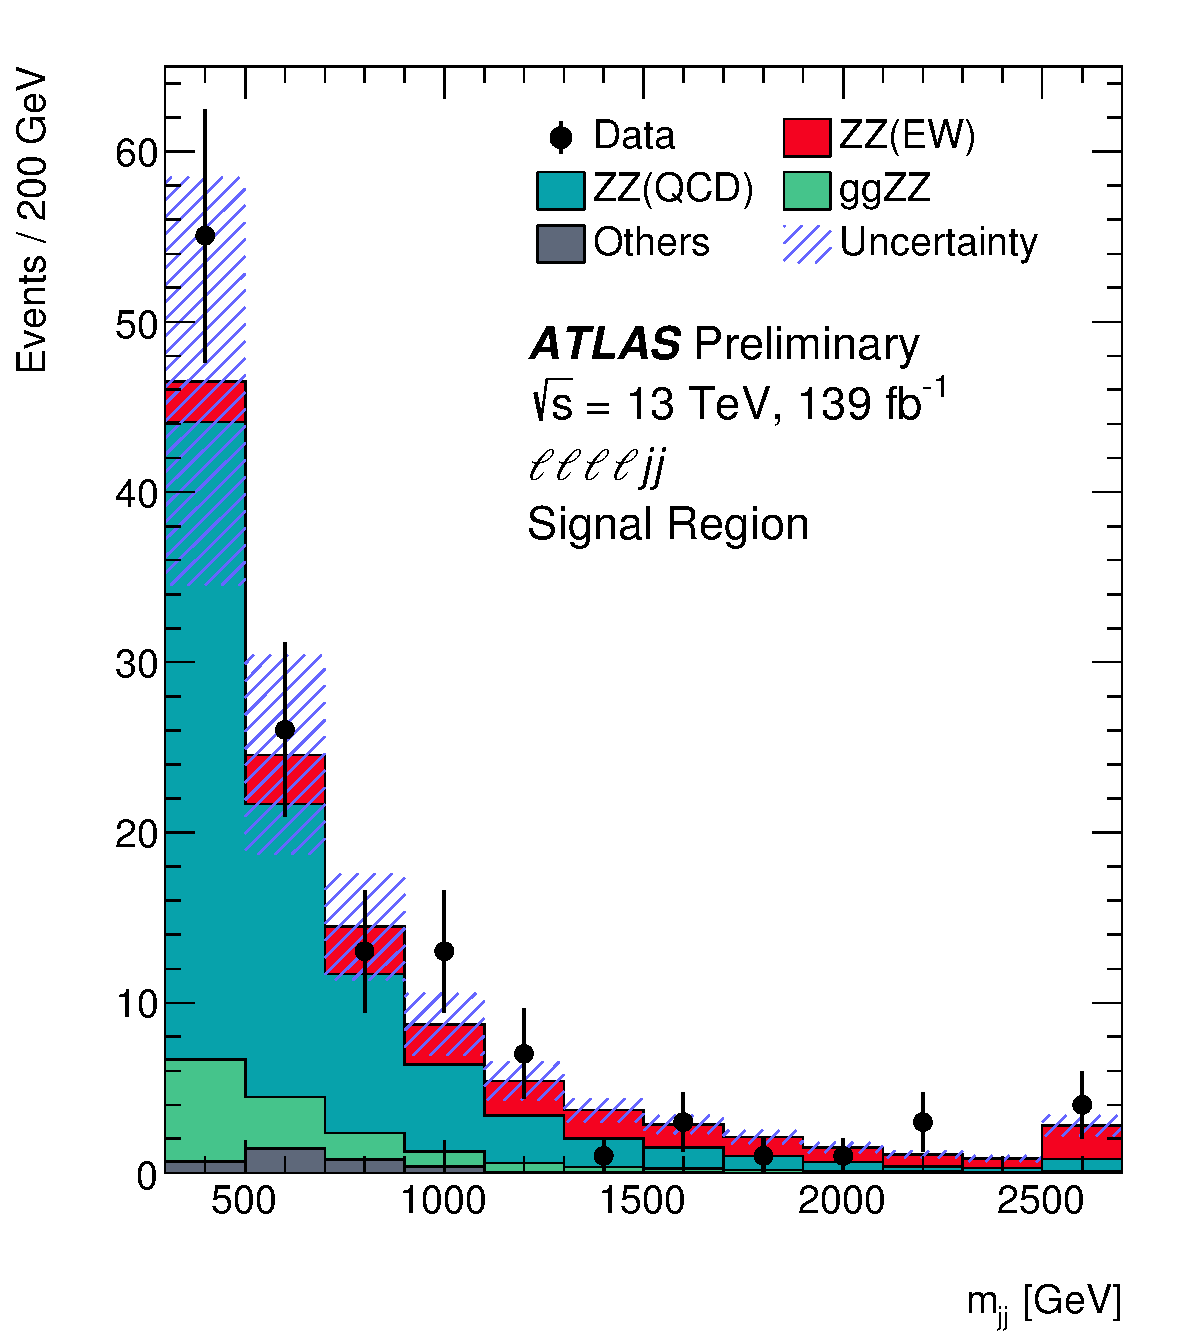
\includegraphics[width=0.32\textwidth]{figures/VBSZZ/fit/MJJ_4l_SR.pdf}
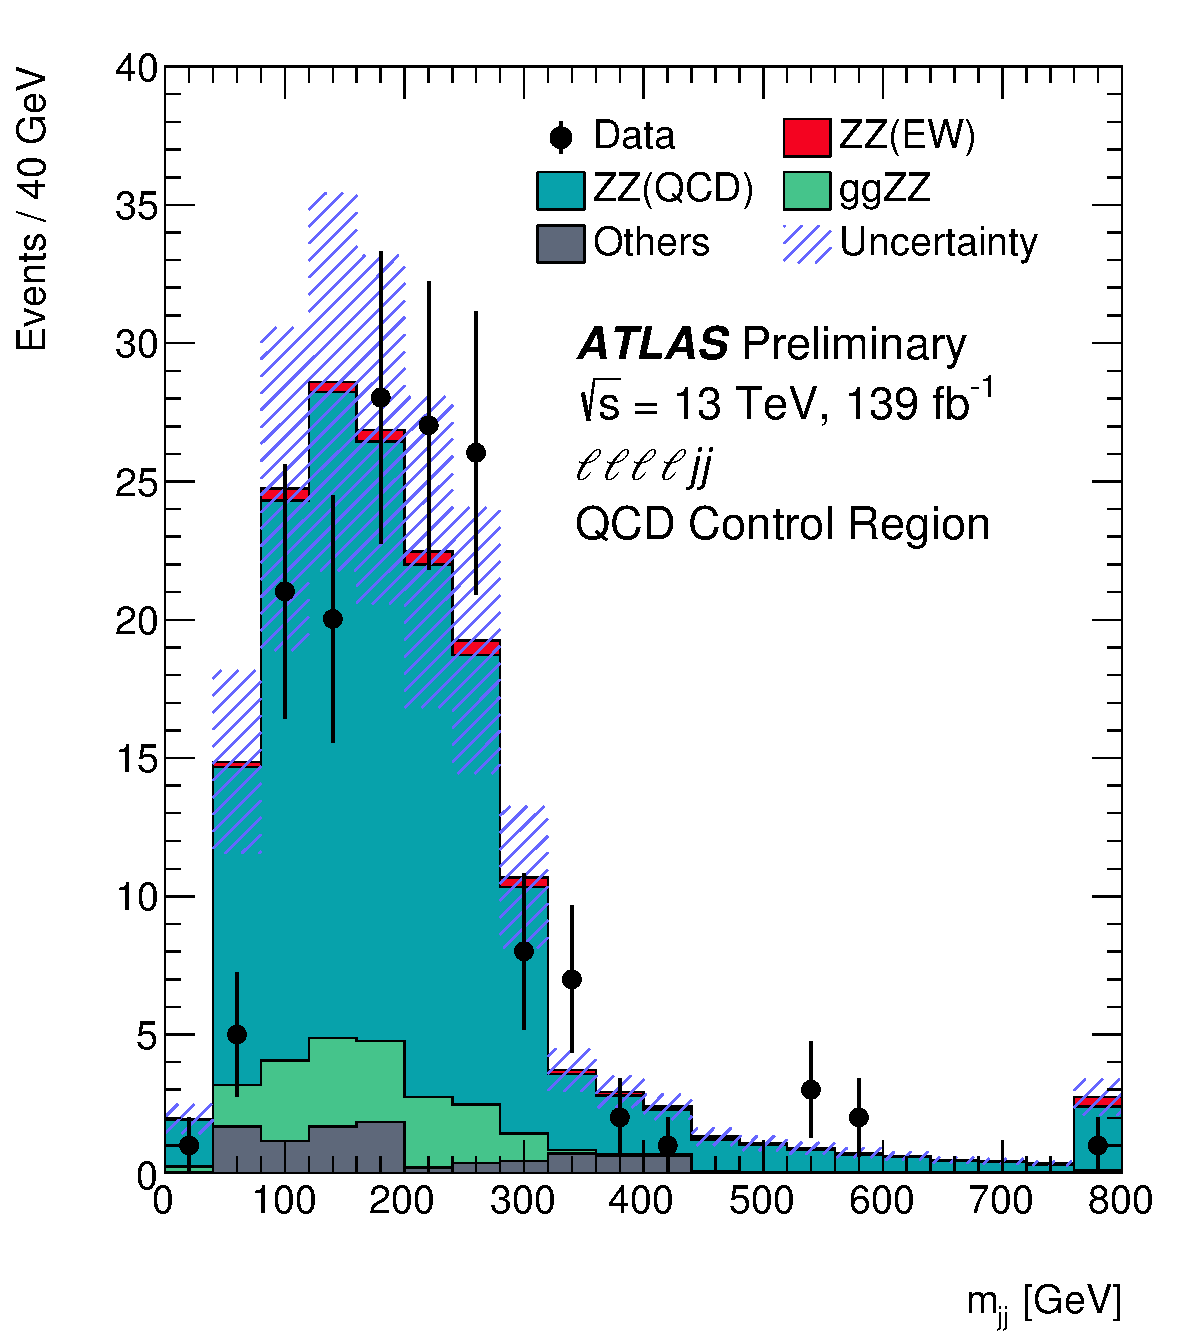
\includegraphics[width=0.32\textwidth]{figures/VBSZZ/fit/MJJ_4l_QCD_CR.pdf}
\end{center}
\caption{Observed and expected \mjj distributions in SR (left) and QCD CR (right).
        The error bands include the expected experimental and theoretical uncertainties.
        The error bars on the data points show the statistical uncertainty on data.
        The contributions from the QCD and EW production of $ZZjj$ events are scaled by 0.96 and 1.35, respectively,
        which correspond to the observed normalization factors in the statistical fit to the combined channel.
        The last bin includes the overflow events.
        }
\label{fig:scaled_mjj}
\end{figure}

\begin{figure}[!htbp]
\begin{center}
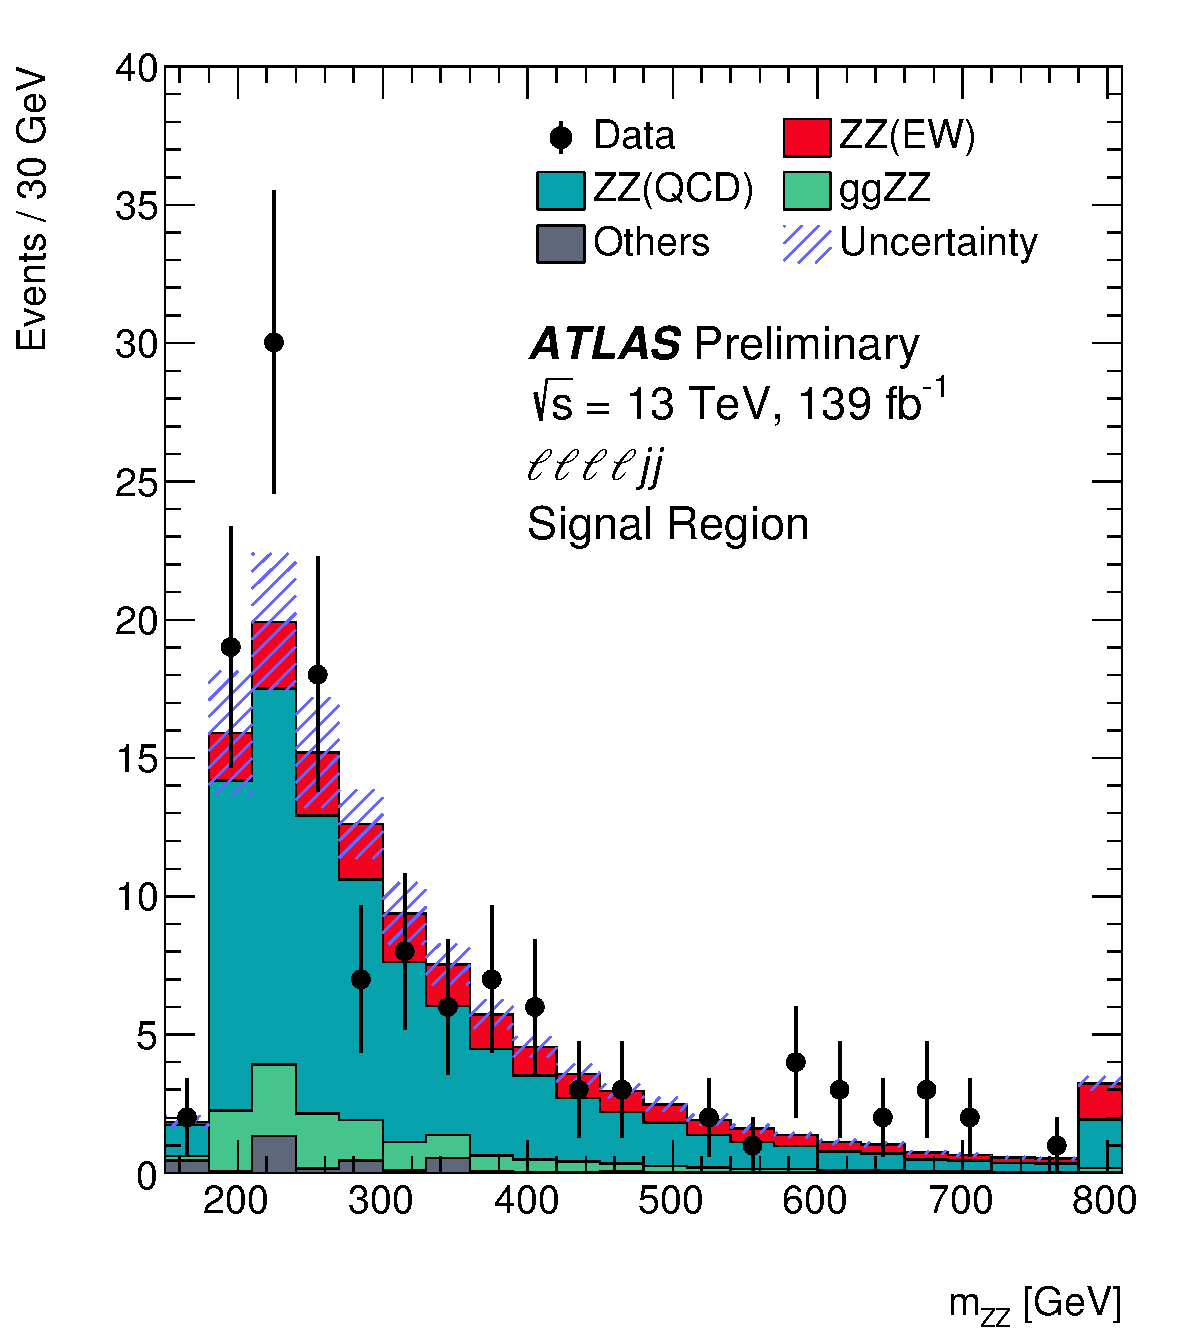
\includegraphics[width=0.4\textwidth]{figures/VBSZZ/fit/MZZ_4l_SR.pdf}
\end{center}
\caption{Observed and expected $\mzz$ spectrum in SR.
        The error bands include the expected experimental and theoretical uncertainties.
        The error bars on the data points show the statistical uncertainty on data.
        The contributions from the QCD and EW production of $ZZjj$ events are scaled by 0.96 and 1.35, respectively,
        which correspond to the observed normalization factors in the statistical fit to the combined channel.
        The last bin includes the overflow events.
        }
\label{fig:scaled_mzz}
\end{figure}

\subsection{MD discriminant}

To further separate the EW-$ZZjj$ component from QCD-$ZZjj$, a MD based on \textit{Gradient Boosted Decision Tree (BDTG)} algorithm\cite{Coadou_BDT} 
is trained with simulated events via TMVA framework\cite{Speckmayer_2010}.
For \llll channel, training is performed between EW (signal) and QCD (background) processes.
Twelve event kinematic variables sensitive to the characteristics of the EW signal is used as input features in training. 
Table~\ref{tab:bdt_features} listed those input variables with the order of their ranking provide by TMVA tool.
The jet-related information provides larger sensitive in \llll final-state.
\begin{table}[h]
\begin{center}
\renewcommand\arraystretch{1.8}
\begin{tabular}{p{1cm}|p{2cm}|p{8cm}}
\hline
\hline
Rank & Variables                    & Description 			\\ \hline
1    & \mjj                         & Dijet invariant mass 		\\ \hline
2    & $p_{T}^{j1}$                 & \pT of the leading jet		\\ \hline
3    & $p_{T}^{j2}$                 & \pT of the sub-leading jet	\\ \hline
4    & $\frac{p_{T}(ZZjj)}{H_{T}(ZZjj)}$  & \pT of the $ZZjj$ system divided by the scalar \pT sum of Z bosons and two jets \\ \hline
5    & $y_{j1} \times y_{j2}$       & Product of jet rapidities		\\ \hline
6    & \dyjj                        & Rapidity difference between two jets \\ \hline
7    & $Y_{Z2}^{*}$                 & Rapidity of the second Z boson \\ \hline
8    & $Y_{Z1}^{*}$                 & Rapidity of the Z boson reconstructed from the lepton pair with the mass closer to the Z boson mass \\ \hline
9    & $p_{T}^{ZZ}$                 & \pT of 4l system \\ \hline
10   & $m_{ZZ}$                     & Invariant mass of 4l system \\ \hline
11   & $p_{T}^{Z1}$                 & \pT of the Z boson reconstructed from the lepton pair with the mass closer to the Z boson mass \\ \hline
12   & $p_{T}^{\ell 3}$             & \pT of the third lepton \\ \hline
\hline
\hline
\end{tabular}
\caption{Input features for the training of MD. }
\label{tab:bdt_features}
\end{center}
\end{table}
Then the MD distributions in both SR and QCD CR region are used for statistical fit.

\subsection{Profile likelihood ratio method}

To examine the compatibility between data and the signal-plus-background hypothesis, 
a test statistic is driven by using the profile likelihood ratio method.
%The likelihood function is the product of all the Poisson probability density functions built in individual MD bins given as:
The binned likelihood function is given as"
\begin{equation}
	\mathcal{L}(\mu,\sigma) = \prod_{i}^\mathrm{bins} \mathcal{L}_{\mathrm{poiss}}(N_{\mathrm{data}}\,|\,\mu s(\theta)+b(\theta))_{i} \times \mathcal{L}_{\text{gauss}}(\theta)_{i}
\end{equation}
where the Poisson term presents the statistical fluctuations of the data 
and a Gaussian term models the pdf of auxiliary measurement to constrain the systematics.
$\mu$ denotes the signal strength of EW-$ZZjj$ process, computed as the ratio between measured (expected) cross section to the SM prediction.
$\theta$ presents the nuisance parameter, which is the set of parameters that parameterize the effect of systematic uncertainties described in section~\ref{sec:systematics}.
$N_{data}$ is the number of selected data events, while the $s(\theta)$ is the expected signal yield and $b(\theta)$ is the expected background yield as the function of nuisance parameters.

The test statistic $q_{\mu}$ is defined as:
\begin{equation}
	q_\mu = -2 \ln \left( \dfrac{\mathcal{L}(\mu,\hat{\hat{\theta}}_{\mu})}{\mathcal{L}(\hat{\mu},\hat{\theta})} \right)
\end{equation}
in which $\mathcal{L}(\hat{\mu},\hat{\theta})$ is the unconditional likelihood with respect to both $\mu$ and $\theta$,
and $\mathcal{L}(\mu,\hat{\hat{\theta}}_{\mu})$ is the conditional likelihood for a constant $\mu$.
Signal-like data distributions are more likely to have a low test-statistic ($q_\mu$ close to 0) 
while the contributions of background-like data have a larger $q_\mu$.
Under the background-only hypothesis, the compatibility of the observed (Asimov) data with the prediction 
is calculated to obtain the observed (expected) significance respectively.

\subsection{Fitting procedure}

A profile likelihood fit is performed on MD discriminant to extract the EW-$ZZjj$ signal from backgrounds.
%The fit combined the observed and expected measurements from both \llll and \llvv channel from EW-ZZ production to gain more statistic.
The binning of MD distributions in SR is optimized to maximize the sensitive for detecting EW signal.
The normalization of QCD-$ZZjj$ production ($\mu_{QCD}^{llll}$) in \llll channel is varied simultaneously in the fit in SR and QCD CR as described in section~\ref{sec:background}.
The signal strength of EW-$ZZjj$ production ($\mu_{EW}$) is taken as parameter of interest and floated in the fit.
The effects of the uncertainties related to normalizations and shapes described previously in section~\ref{sec:systematics} 
of background processes in the MD distribution are all taken into account.

In most case, a common nuisance parameter is used for each source of systematic in all bins and all channels.
The statistical uncertainties for simulated samples are uncorrelated among all bins, and the background uncertainties only applied to their corresponding backgrounds.
For combination between two channels, the theoretical uncertainties between \llll and \llvv are uncorrelated due to different fiducial volumes definition.
Furthermore, to be more conservative, the generator modelling uncertainty for QCD-$ZZjj$ production mentioned in section~\ref{sec:systematics}
is separated to be two nuisance parameters in low and high MD region.

\subsection{Result of statistical fit}

The statistical fit is performed both in individual \llll channel, as well as the combination between \llll and \llvv channel to gain more statistic.
The results of statistical fit for \llll channel and the combined channel are presented in table~\ref{tab:fit_result}.
The \llvv analysis will not be talked about in this thesis, but more details can refer to \cite{ATLAS:2019vrv}.
To drive expected results, the observed data is used for QCD CR to extract normalization factor of QCD component ($\mu_{QCD}^{llll}$),
while in SR, asimov data built from background prediction and signal model with SM assumed cross section is used.
\begin{table}[!htbp]
\begin{center}
\begin{tabular}{c|c|c|c}
\hline
                 & $\mu_{\mathrm{EW}}$ &  $\mu^{\lllljj}_{\mathrm{QCD}}$   &  Significance Obs. (Exp.) \\
\hline
\lllljj          & $1.54 \pm 0.42$     &  $0.95 \pm 0.22$                  &  5.48 (3.90) $\sigma$     \\
\hline
Combined         & $1.35 \pm 0.34$     &  $0.96 \pm 0.22$                  &  5.52 (4.30) $\sigma$     \\
\hline
\end{tabular}
\end{center}
\caption{
Observed \muEW and \muQCD, as well as the observed and expected significance from the individual \lllljj channel, and the combined fits.
The full set of systematic uncertainties is included.
}
\label{tab:fit_result}
\end{table}
For \llll channel, the background-only hypothesis is rejected at 5.5$\sigma$ (3.9$\sigma$) for data (expectation),
which leads to the observation of EW-$ZZjj$ production.
Figure~\ref{fig:fit_MD} shows the post-fit MD distributions for \llll channel in SR (left) and QCD CR (right).
The EW-$ZZjj$ cross section measured in \llll channel is extracted to be $0.94 \pm 0.26$~fb.
\begin{figure}[!htbp]
\begin{center}
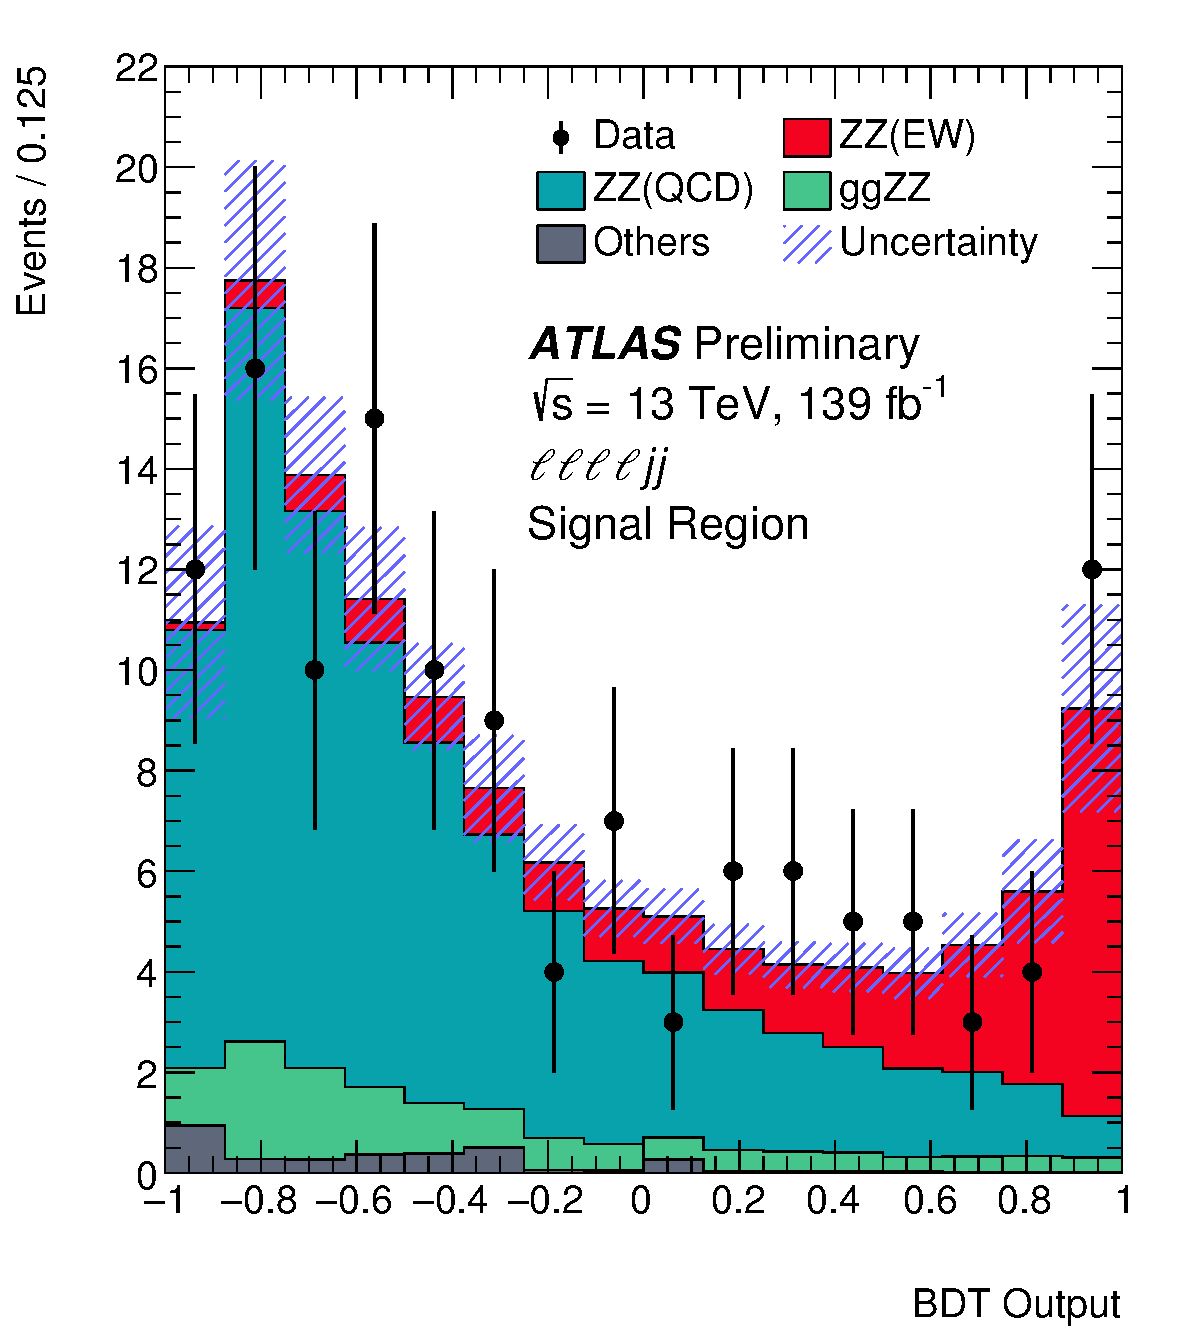
\includegraphics[width=0.42\textwidth]{figures/VBSZZ/fit/BDT_4l_SR_postFit.pdf}
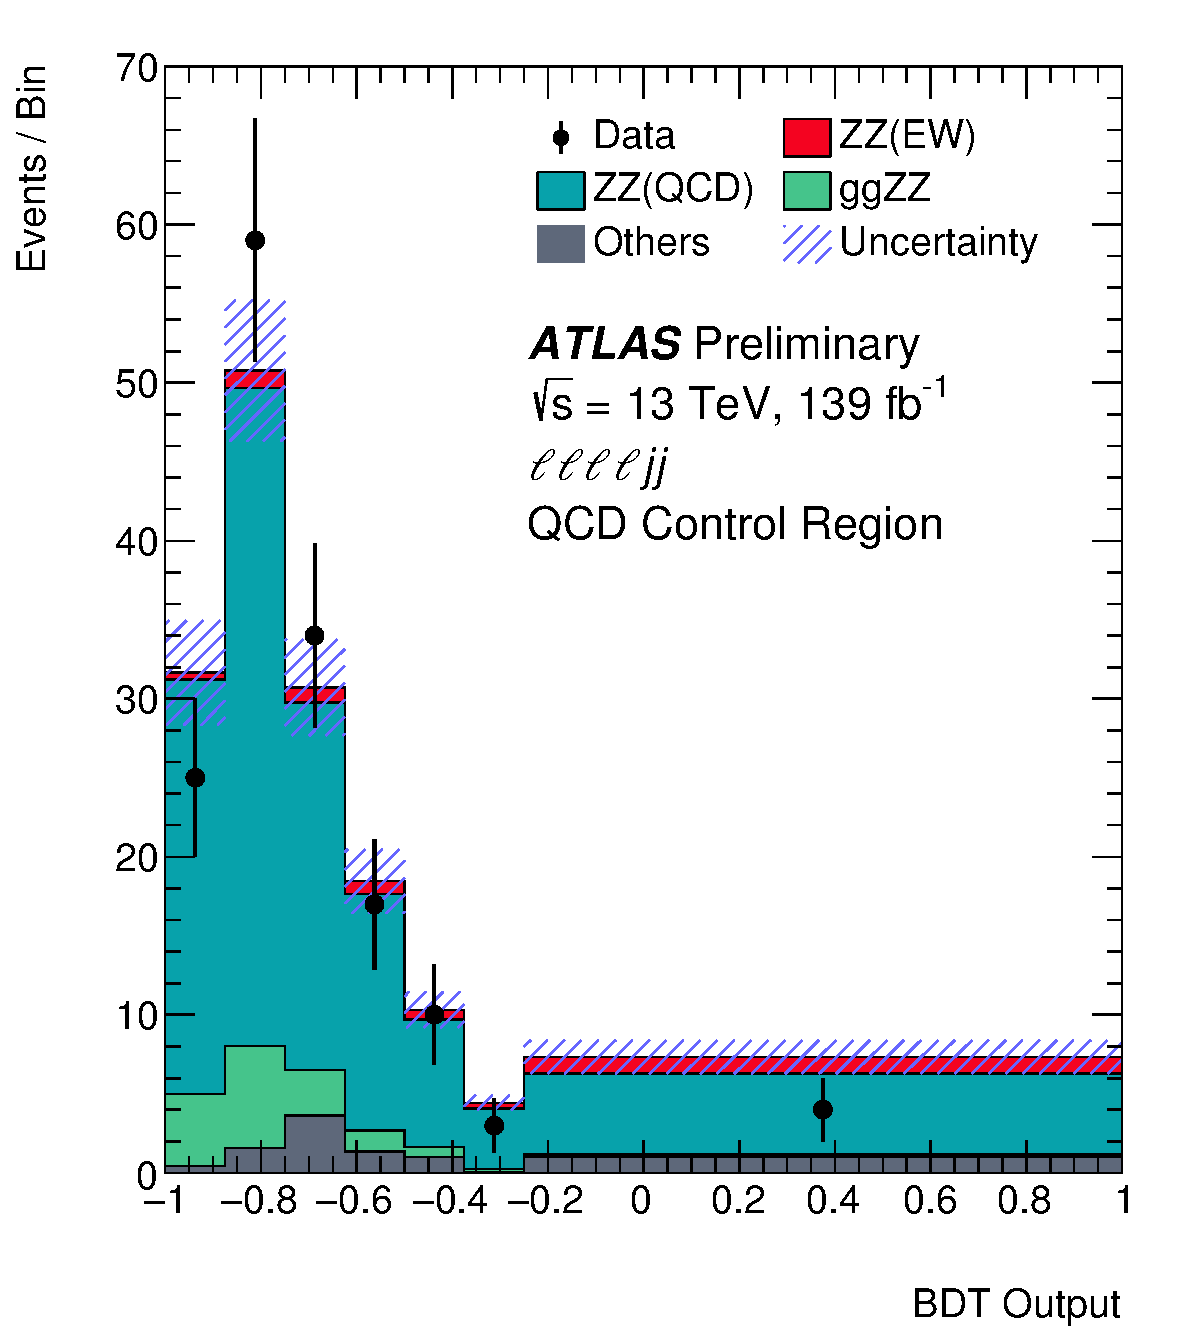
\includegraphics[width=0.42\textwidth]{figures/VBSZZ/fit/BDT_4l_QCD_CR_postFit.pdf}
\end{center}
\caption{Observed and expected multivariate discriminant distributions after the statistical fit in the \llll SR (left) and QCD CR (right).
        The error bands include the experimental and theoretical uncertainties,
        as well as the uncertainties in \muEW and \muQCD.
        The error bars on the data points show the statistical uncertainty on data.
        }
\label{fig:fit_MD}
\end{figure}

Figure~\ref{fig:event_display} depicts the display of an event candidate of EW-$ZZjj$ production in $2e2\mu$ final state with two jets in forward and backward region, and with a MD value from 0.875 to 1.0.
\begin{figure}[!htbp]
\begin{center}
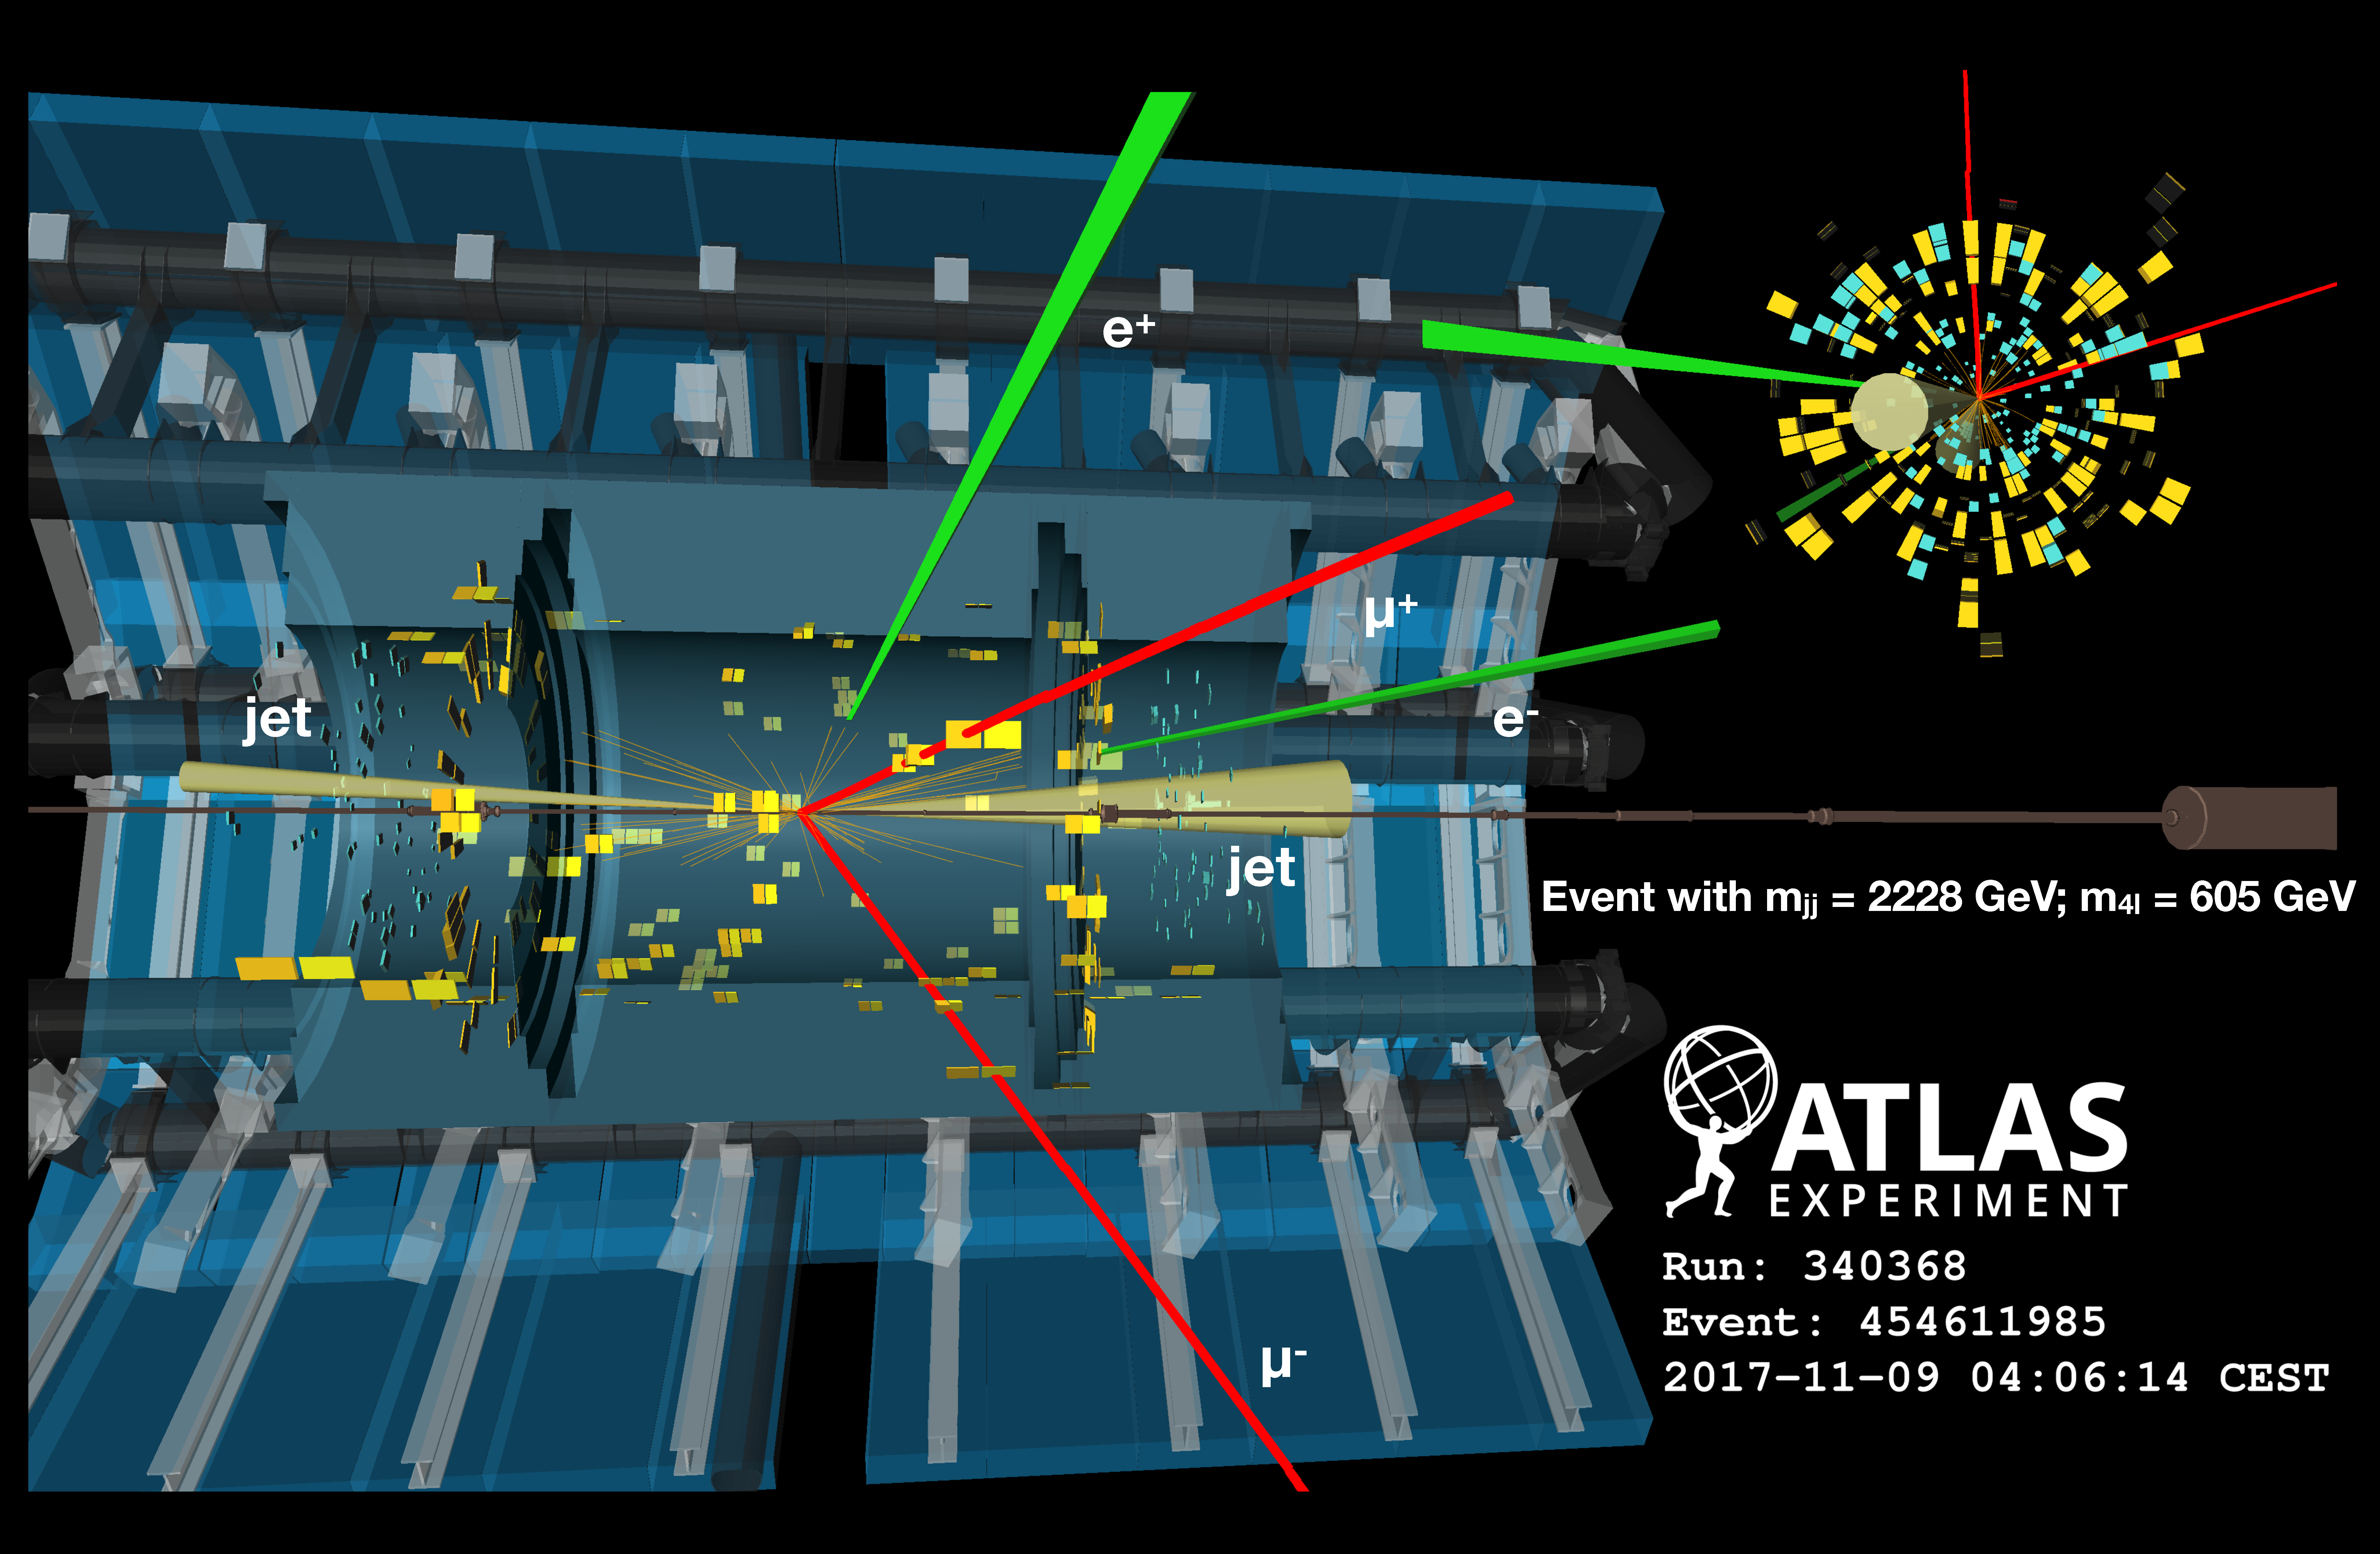
\includegraphics[width=1.0\textwidth]{figures/VBSZZ/fit/resize_340368_454611985_v3.pdf}
\end{center}
\caption{Display of an event candidate of EW-$ZZjj$ production in $2e2\mu$ channel in last MD bin (0.875 < MD < 1.0).
         The invariant mass of the di-jet (four-lepton) system is 2228 (605)~\gev. }
\label{fig:event_display}
\end{figure}
